% %%%%%%%%%%%%%%%%%%%%%%%%%%%%%%%%%%%%%%%%%%%%%%%%%%%%%%%%%%%%%%%%%%%%%%%%%%%%%
% %%%%%%%%%%%%%%%%%%%%%%%%%%%%%%%%%%%%%%%%%% Results with Respect to Modenumber
% %%%%%%%%%%%%%%%%%%%%%%%%%%%%%%%%%%%%%%%%%%%%%%%%%%%%%%%%%%%%%%%%%%%%%%%%%%%%%

\chapter{Large Modenumber Effects}
\label{ch_bigm}

This is why we do 2.5D... you can't resolve these effects in a 3D model. It's too expensive. 

\todo{Do we see a difference between \vec{k} (momentum) and the group velocity? Poynting flux will always be pretty much along the field line, since $B_3$ is small and $E_3$ is zero, but the wave vector need not be. This is a question of coupling/converting to compressional waves, I guess. }

\todo{Look at McKenzie and Westphal. Waves incident on the bow shock, etc, at weird angles. }

\todo{Look at the E to B ratio. Compare to the \Alfven speed and to the height-integrated Pedersen conductivity. }

% =============================================================================
% =============================================================================
% =============================================================================
\section{Finite Poloidal Lifetimes}

Radoski 1974 \cite{radoski_1974}. Ding 1995\cite{ding_1995}. Mann 1995\cite{mann_1995}. 

\todo{Look at Mann's poloidal lifetime, $\dd{\omega_A'} \lambda$ where $\lambda \sim \frac{\azm}{2 \pi r}$. }

\begin{figure}[H]
    \centering
    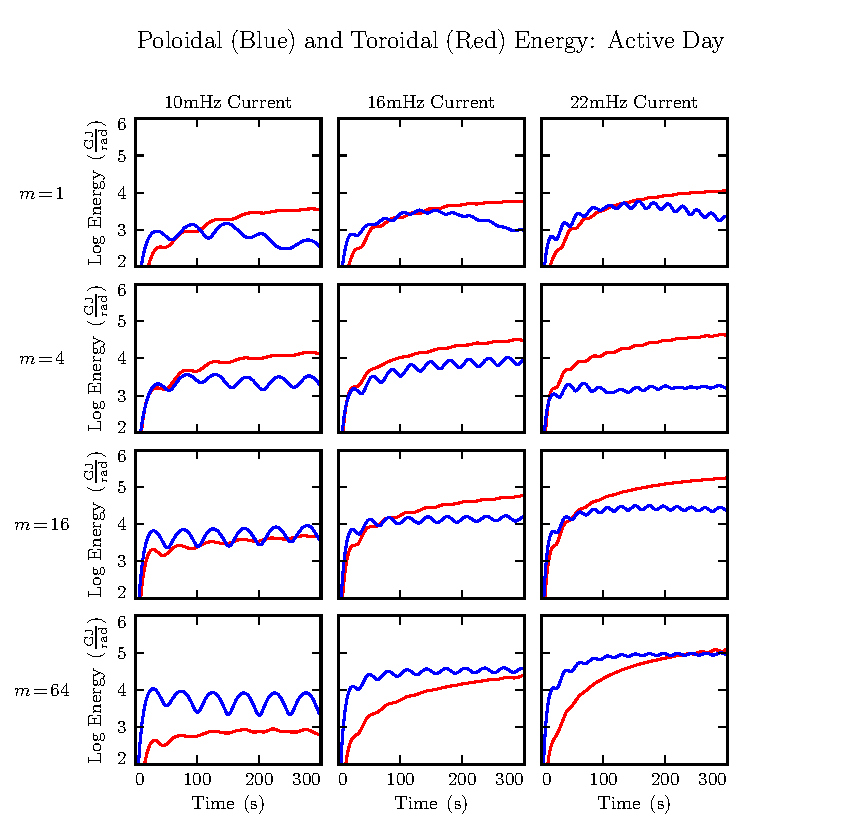
\includegraphics[width=\textwidth]{figures/UP_UT_J_1.pdf}
    \caption[Current-Driven Poloidal and Toroidal Energy: Active Day]{}
    \label{fig_UP_UT_J_1}
\end{figure}

\begin{figure}[H]
    \centering
    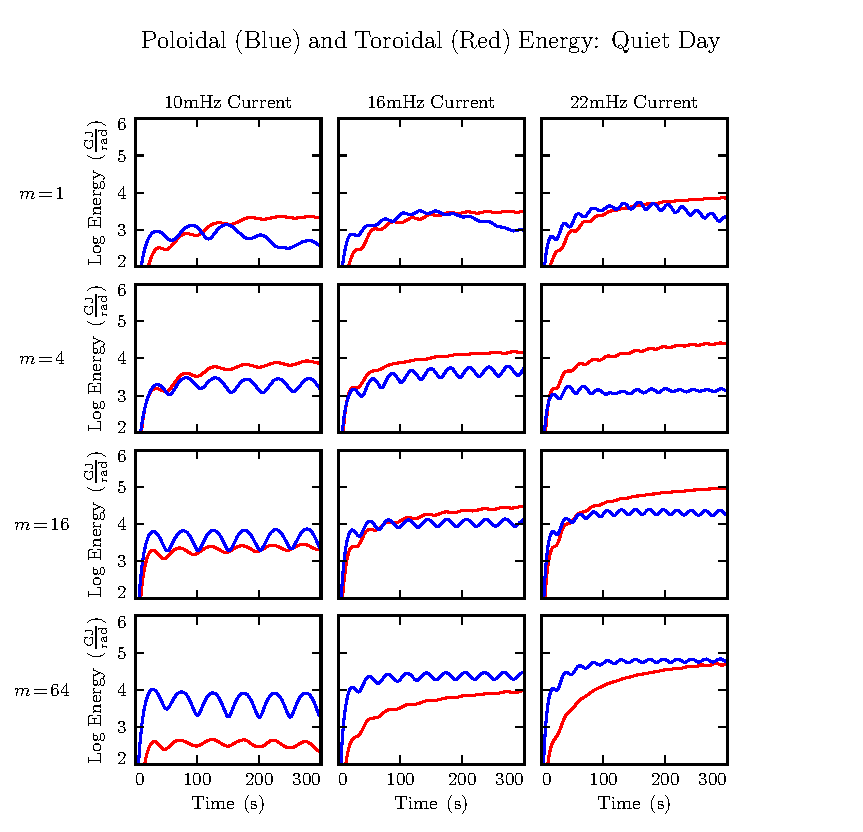
\includegraphics[width=\textwidth]{figures/UP_UT_J_2.pdf}
    \caption[Current-Driven Poloidal and Toroidal Energy: Quiet Day]{}
    \label{fig_UP_UT_J_2}
\end{figure}

\begin{figure}[H]
    \centering
    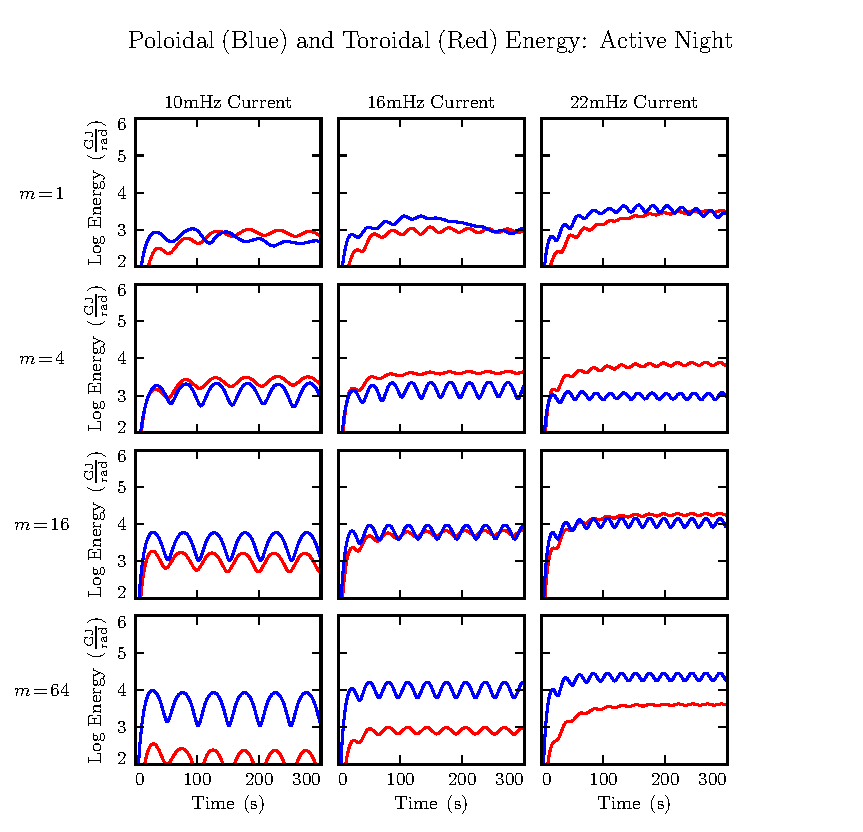
\includegraphics[width=\textwidth]{figures/UP_UT_J_3.pdf}
    \caption[Current-Driven Poloidal and Toroidal Energy: Active Night]{}
    \label{fig_UP_UT_J_3}
\end{figure}

\begin{figure}[H]
    \centering
    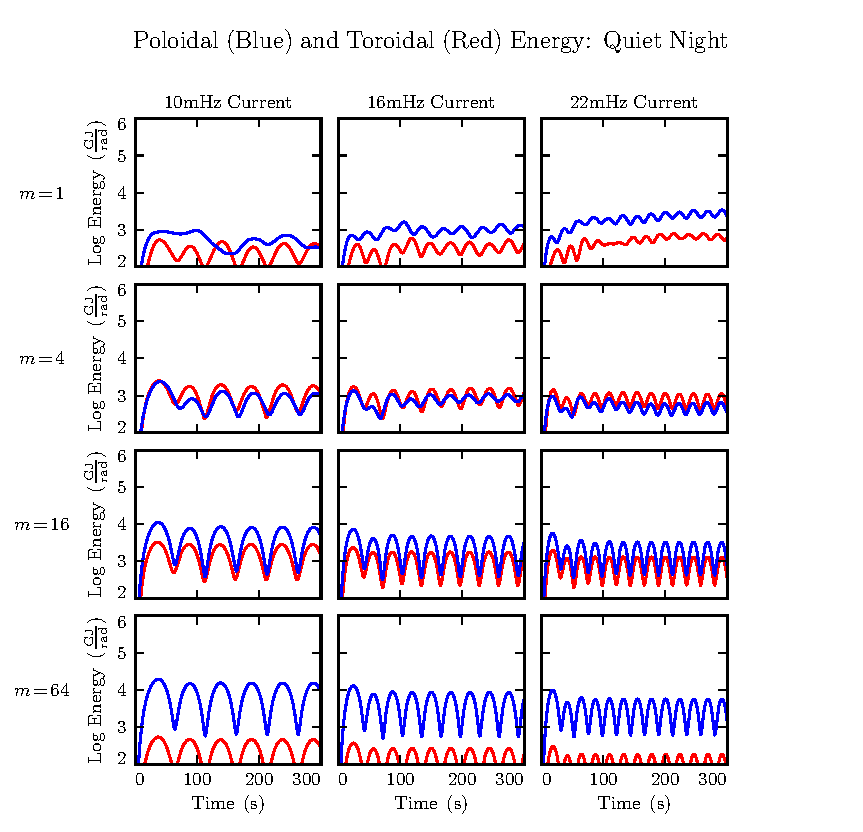
\includegraphics[width=\textwidth]{figures/UP_UT_J_4.pdf}
    \caption[Current-Driven Poloidal and Toroidal Energy: Quiet Night]{}
    \label{fig_UP_UT_J_4}
\end{figure}

%\begin{figure}[H]
%    \centering
%    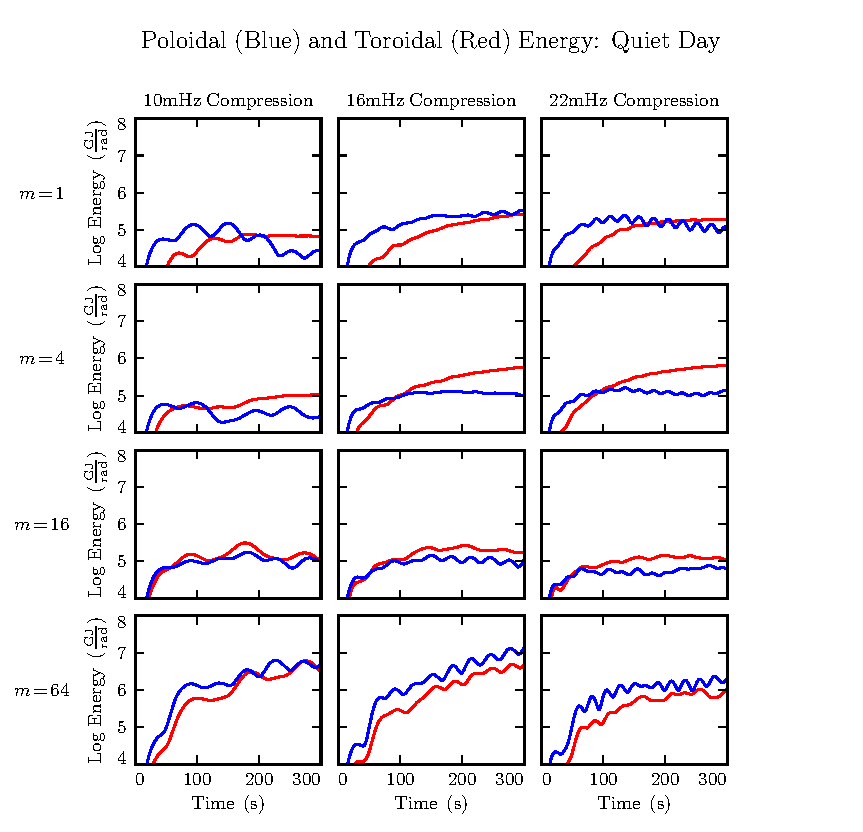
\includegraphics[width=\textwidth]{figures/UP_UT_B_2.pdf}
%    \caption[Compression-Driven Poloidal and Toroidal Energy: Quiet Day]{}
%    \label{fig_UP_UT_B_2}
%\end{figure}

%\begin{figure}[H]
%    \centering
%    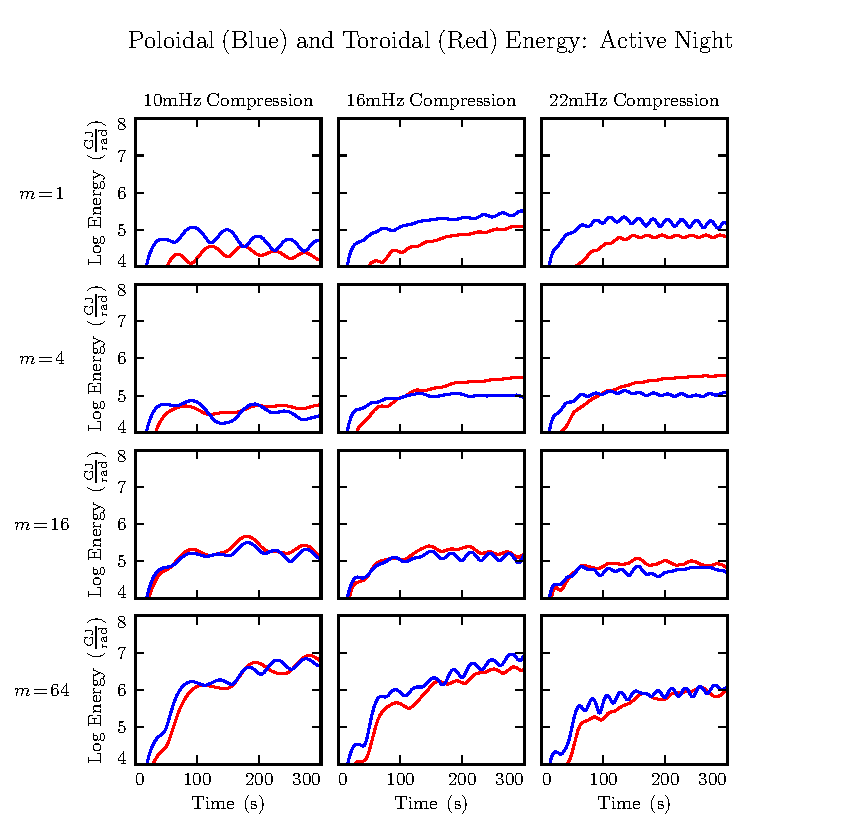
\includegraphics[width=\textwidth]{figures/UP_UT_B_3.pdf}
%    \caption[Compression-Driven Poloidal and Toroidal Energy: Active Night]{}
%    \label{fig_UP_UT_B_3}
%\end{figure}

% =============================================================================
% =============================================================================
% =============================================================================
\section{Development of Fine Structure}

% =============================================================================
% =============================================================================
% =============================================================================
\section{Ground Signatures}

East-west fields. 

\begin{figure}[H]
    \centering
    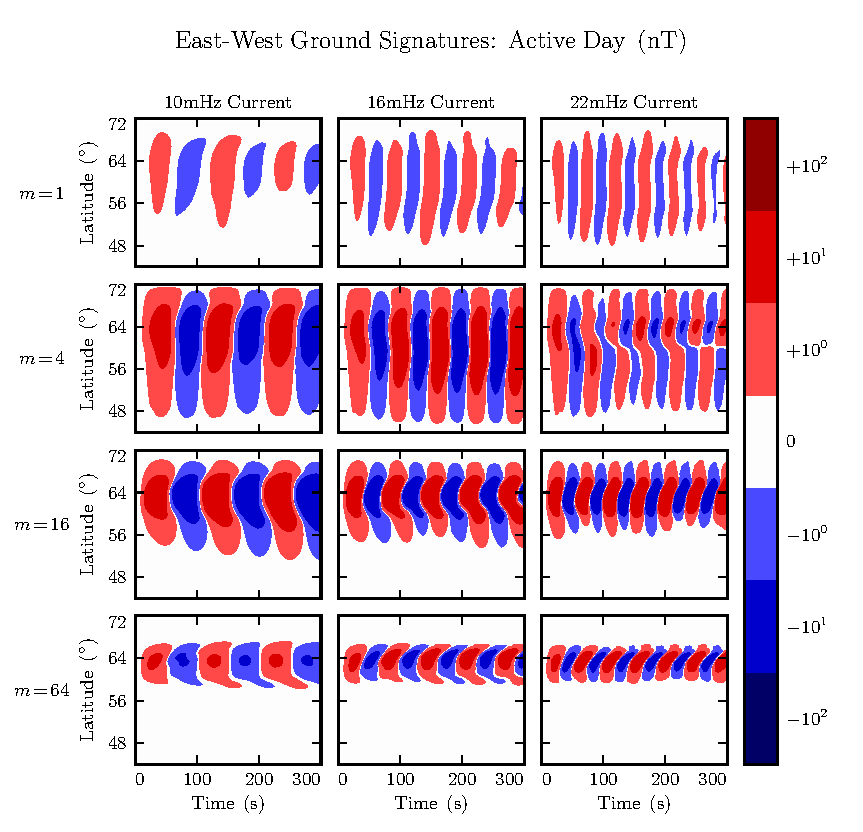
\includegraphics[width=\textwidth]{figures/BfE_J_1.pdf}
    \caption[East-West Ground Signatures: Active Day]{}
    \label{fig_BfE_J_1}
\end{figure}

\begin{figure}[H]
    \centering
    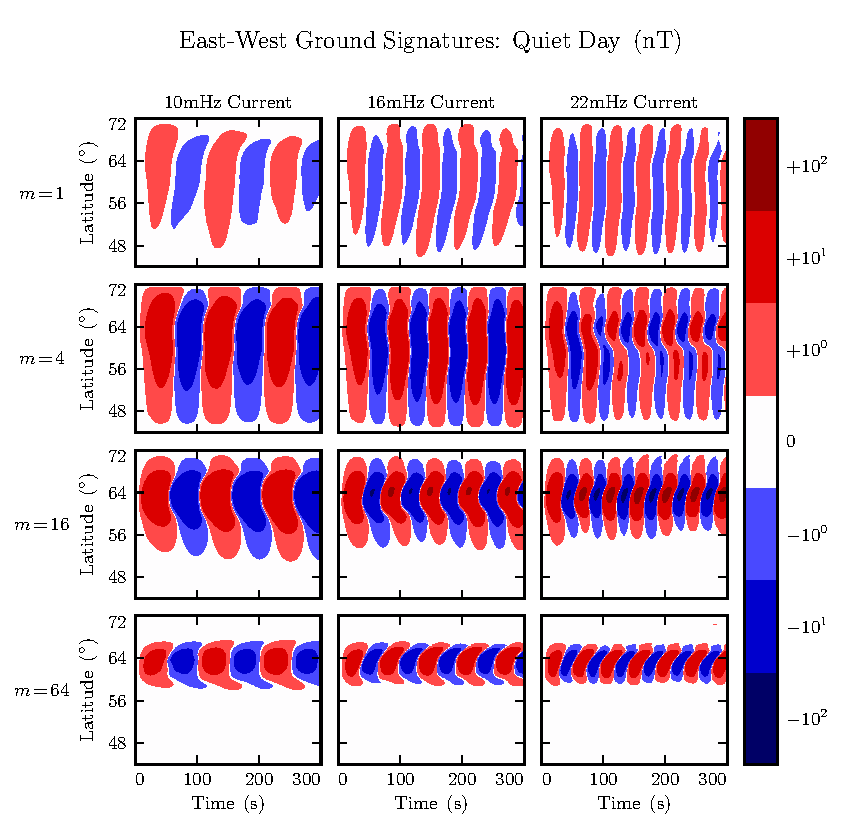
\includegraphics[width=\textwidth]{figures/BfE_J_2.pdf}
    \caption[East-West Ground Signatures: Quiet Day]{}
    \label{fig_BfE_J_2}
\end{figure}

\begin{figure}[H]
    \centering
    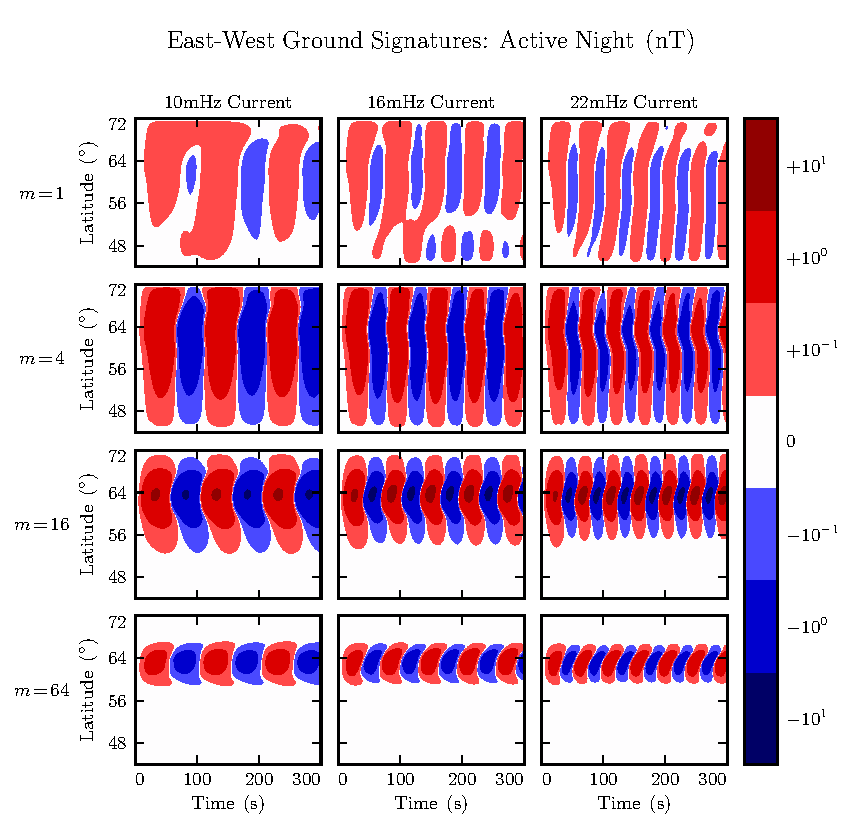
\includegraphics[width=\textwidth]{figures/BfE_J_3.pdf}
    \caption[East-West Ground Signatures: Active Night]{}
    \label{fig_BfE_J_3}
\end{figure}

\begin{figure}[H]
    \centering
    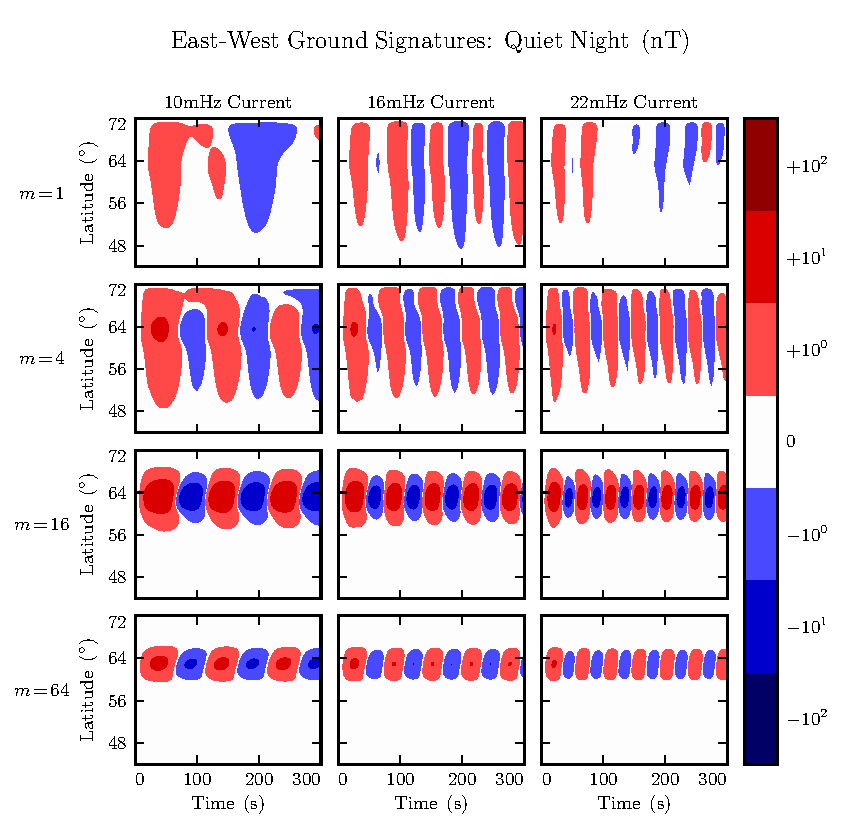
\includegraphics[width=\textwidth]{figures/BfE_J_4.pdf}
    \caption[East-West Ground Signatures: Quiet Night]{}
    \label{fig_BfE_J_4}
\end{figure}

North-south fields. 


\begin{figure}[H]
    \centering
    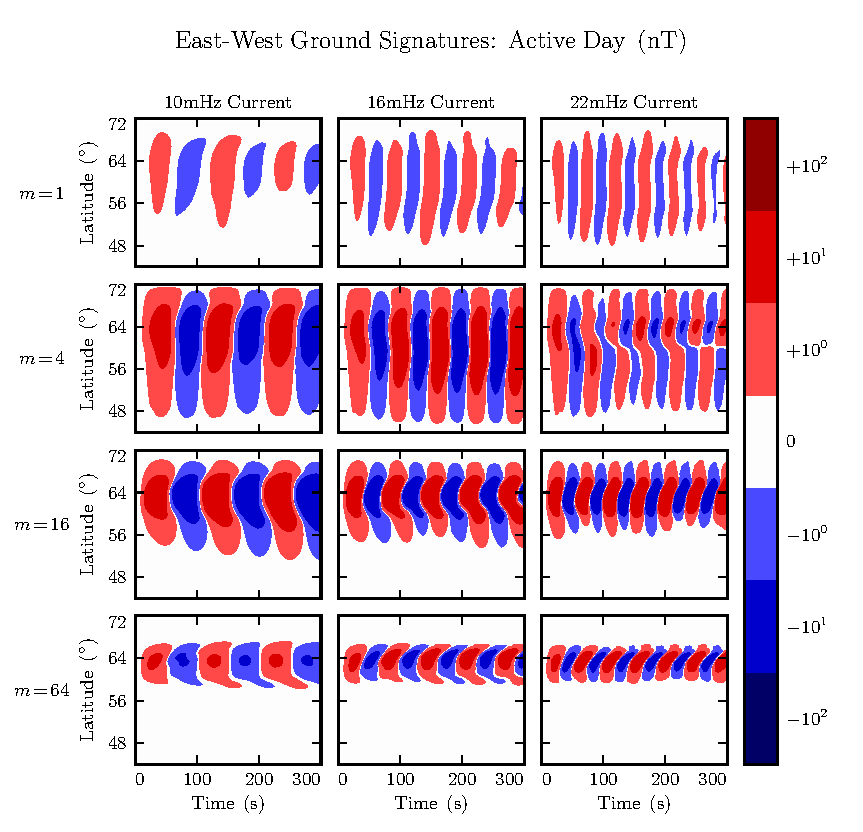
\includegraphics[width=\textwidth]{figures/BfE_J_1.pdf}
    \caption[North-South Ground Signatures: Active Day]{}
    \label{fig_BqE_J_1}
\end{figure}

\begin{figure}[H]
    \centering
    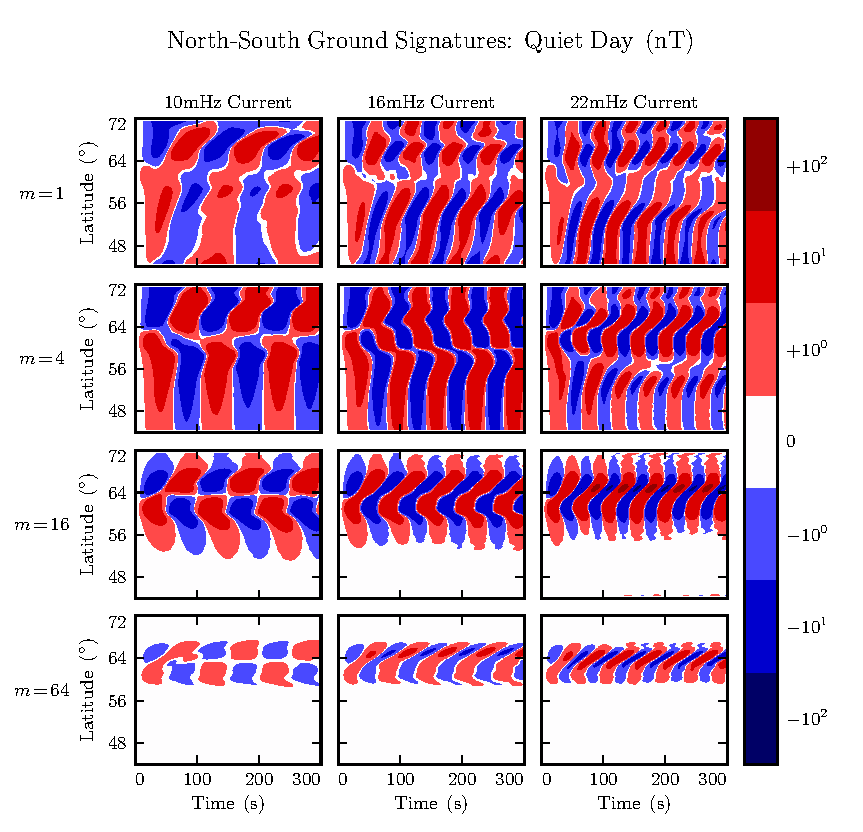
\includegraphics[width=\textwidth]{figures/BqE_J_2.pdf}
    \caption[North-South Ground Signatures: Quiet Day]{}
    \label{fig_BqE_J_2}
\end{figure}

\begin{figure}[H]
    \centering
    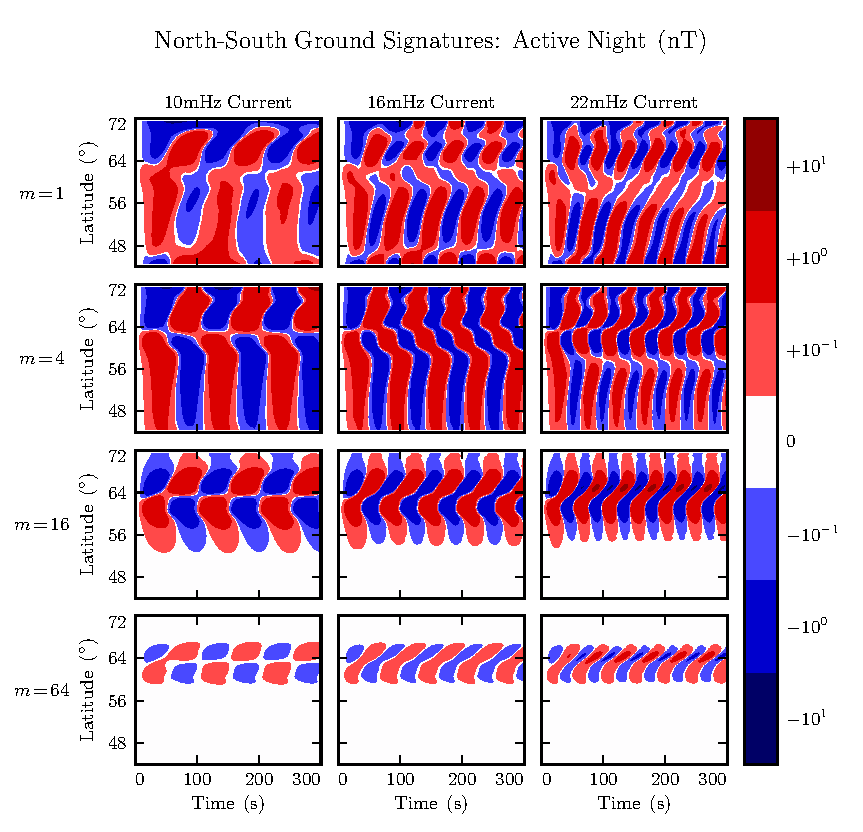
\includegraphics[width=\textwidth]{figures/BqE_J_3.pdf}
    \caption[North-South Ground Signatures: Active Night]{}
    \label{fig_BqE_J_3}
\end{figure}

\begin{figure}[H]
    \centering
    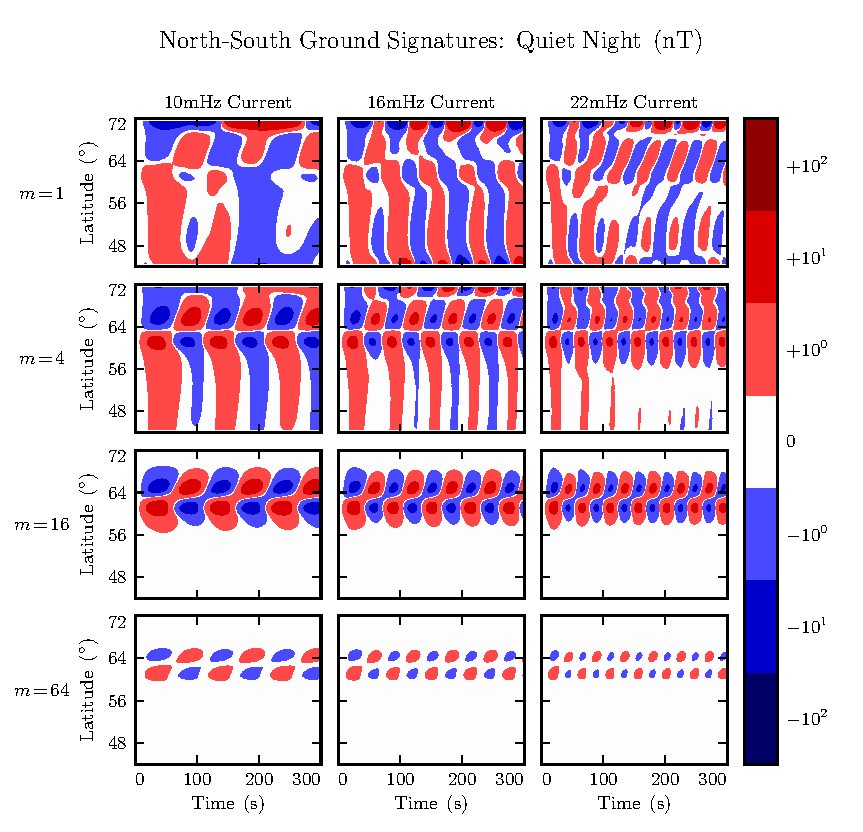
\includegraphics[width=\textwidth]{figures/BqE_J_4.pdf}
    \caption[North-South Ground Signatures: Quiet Night]{}
    \label{fig_BqE_J_4}
\end{figure}






% =============================================================================
% =============================================================================
% =============================================================================
\section{Electromagnetic Energy Gap}


\begin{figure}[H]
    \centering
    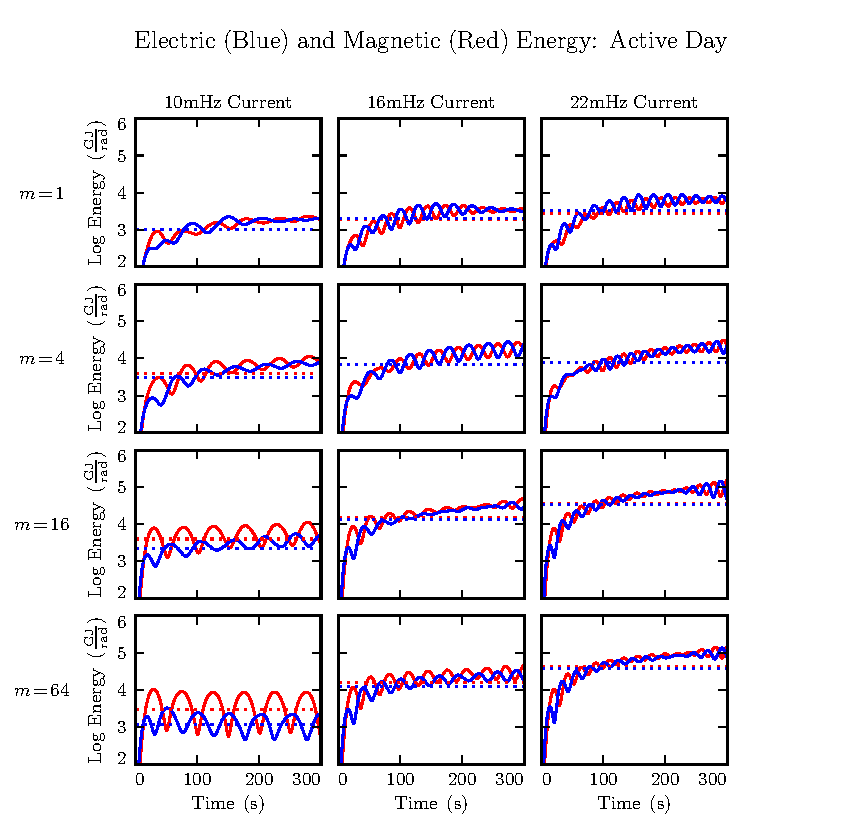
\includegraphics[width=\textwidth]{figures/UB_UE_J_1.pdf}
    \caption[Current-Driven Electric and Magnetic Energy: Active Day]{}
    \label{fig_UB_UE_J_1}
\end{figure}

\begin{figure}[H]
    \centering
    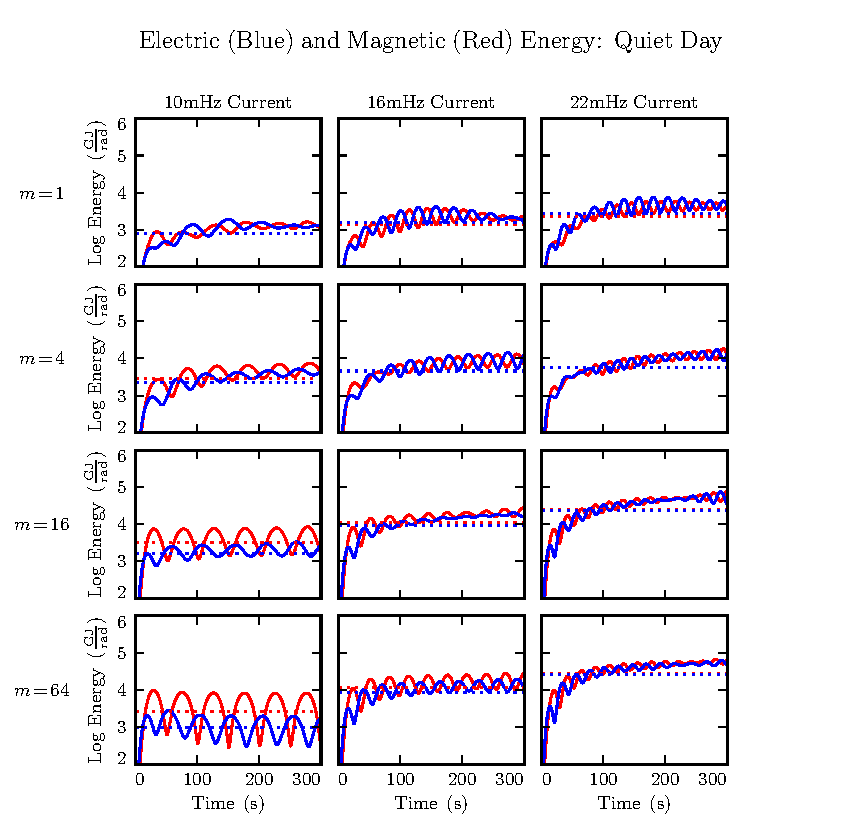
\includegraphics[width=\textwidth]{figures/UB_UE_J_2.pdf}
    \caption[Current-Driven Electric and Magnetic Energy: Quiet Day]{}
    \label{fig_UB_UE_J_2}
\end{figure}

\begin{figure}[H]
    \centering
    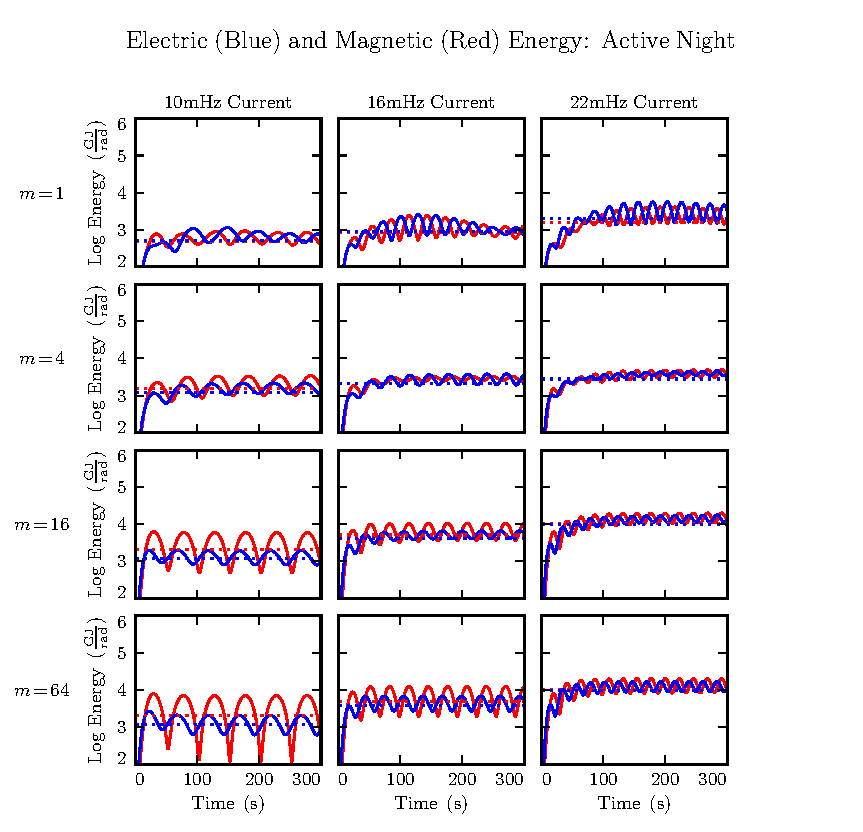
\includegraphics[width=\textwidth]{figures/UB_UE_J_3.pdf}
    \caption[Current-Driven Electric and Magnetic Energy: Active Night]{}
    \label{fig_UB_UE_J_3}
\end{figure}

\begin{figure}[H]
    \centering
    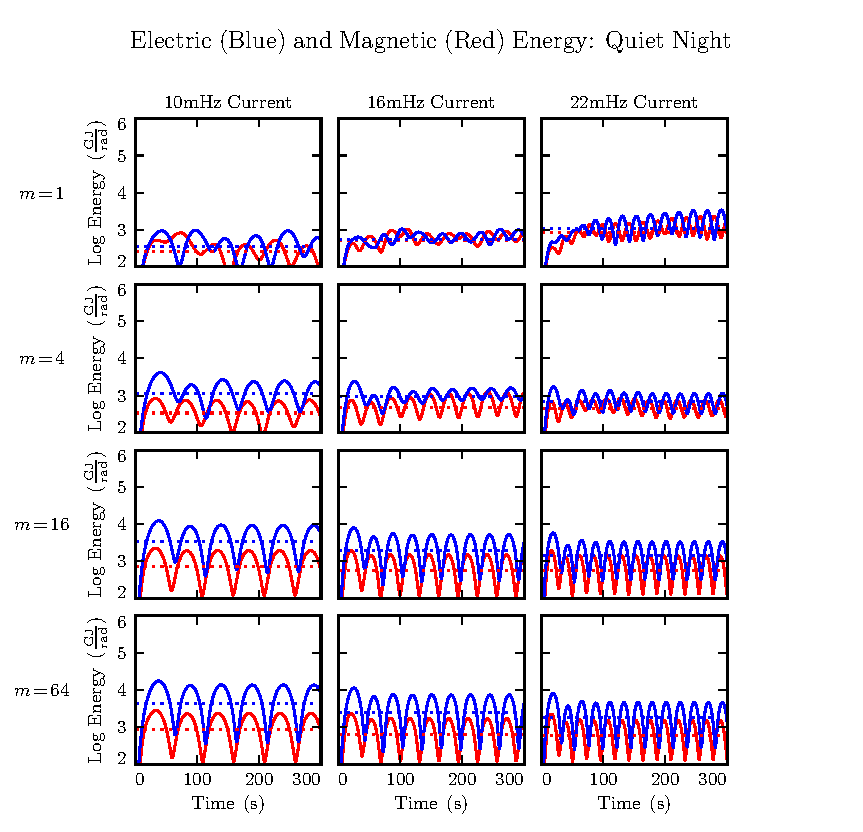
\includegraphics[width=\textwidth]{figures/UB_UE_J_4.pdf}
    \caption[Current-Driven Electric and Magnetic Energy: Quiet Night]{}
    \label{fig_UB_UE_J_4}
\end{figure}








%\begin{figure}[H]
%    \centering
%    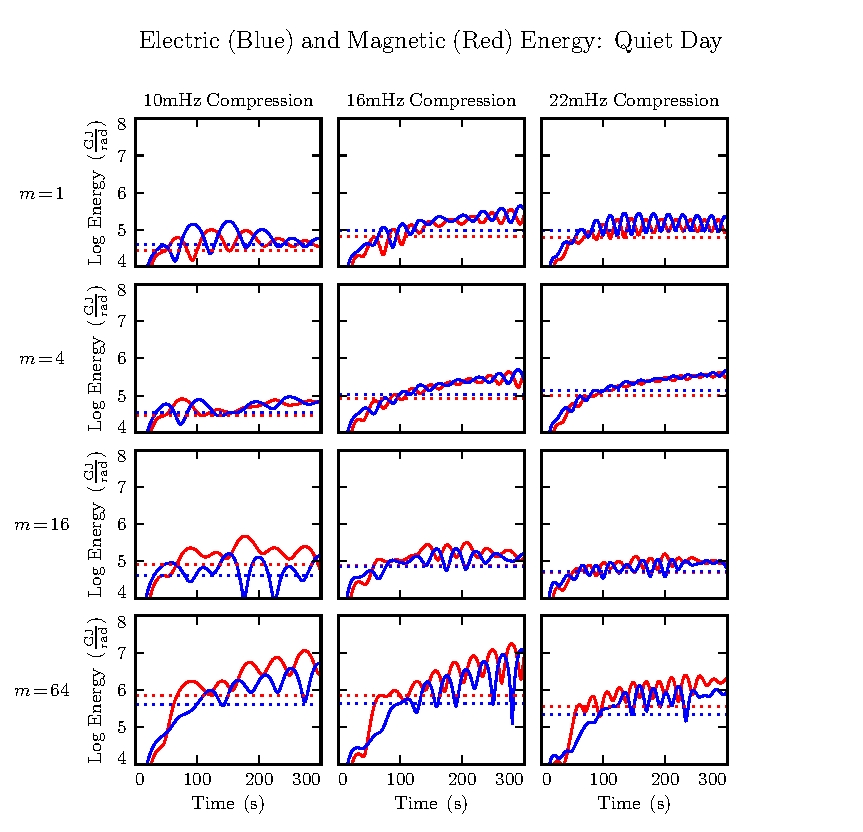
\includegraphics[width=\textwidth]{figures/UB_UE_B_2.pdf}
%    \caption[Compression-Driven Electric and Magnetic Energy: Quiet Day]{}
%    \label{fig_UB_UE_B_2}
%\end{figure}

%\begin{figure}[H]
%    \centering
%    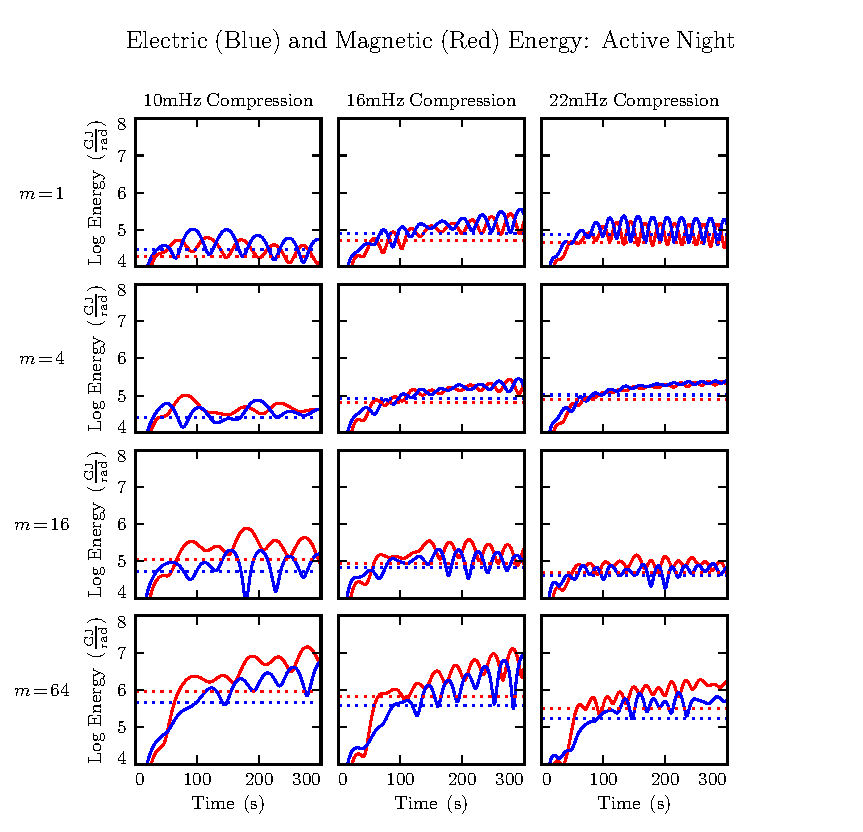
\includegraphics[width=\textwidth]{figures/UB_UE_B_3.pdf}
%    \caption[Compression-Driven Electric and Magnetic Energy: Active Night]{}
%    \label{fig_UB_UE_B_3}
%\end{figure}











